\documentclass[]{article}
\usepackage{graphicx}
\usepackage{amsmath}


%opening
\title{Water Reconstruction Review: Impact of Vertex Uncertainties}
\author{Ed Leming, Nuno Barros}

\begin{document}

\maketitle

\begin{abstract}
This document is intended to summarise the required accuracy of our reconstruction algorithms in the context of the leading analysis from Water Phase.
\end{abstract}

\section{Reconstruction for Nucleon Decay}
M Askins \cite{MorganTalk} has previously produced some plots which show the relative sensitivity of the nucleon decay likelihood analysis as a function of energy, position and direction uncertainties of the reconstructed event vertex. The parameters used to define the systematic in these plots are not identical to those given in the reconstruction section of \cite{WaterUniDoc}. This document is intended to translate between the two in order to give reviewers some context on how reconstruction uncertainties are affecting our leading analyses.

\subsection{Position systematics}
The first thing to note when looking at Figure~\ref{fig:position} is that our ND sensitivity is flat as a function of vertex position until 100~mm or so. With that in mind lets consider the very worst case from the position systematics given in \cite{WaterUniDoc}, i.e. the z axis. This axis shows the largest systematics in all three of the vertex scale, shift and resolution systematics. A reduced accuracy in this plane is expected due to the enhanced detector asymmetries relative to the x and y. A summary of all three position systematics for the z plane is given in Table~\ref{tab:position}. 

\begin{table}
	\label{tab:position}
	\centering
\begin{tabular}{p{2.5cm}|p{3.5cm}}
	\hline
	Systematic &  Value\\
	\hline
	\hline
	Z shift & +42.5 / +16.5~mm \\
	Z scale & +0.03 / -0.37~\%\\
	Z resolution & 13.1~mm\\
	\hline
\end{tabular}
\caption{Vertex position systematics for the z axis, taken from \cite{WaterUniDoc}}
\end{table}

To apply the z-scale systematic, and hence convert into mm units, we use the following equation:
\begin{equation}
z' = (1 - \delta / 100)\cdot z
\end{equation}
therefore to find a range (in mm) at the edge of our fiducial volume we can say:
\begin{alignat}{2}
z_{upper} = (1 + 0.03/100)\cdot 5500 = 5501~mm \\
z_{lower} = (1 - 0.37/100)\cdot 5500 = 5480~mm.
\end{alignat}
the full range at the edge of the fiducial volume is therefore:
\begin{equation}
z^{scale}_{FV} = z_{upper} - z_{lower} = 21~mm
\end{equation}
Finally, taking the squared sum of all three position systematics at the edge of the fiducial volume we can find the total vertex position uncertainty:
\begin{equation}
\Delta_{position} = \sqrt{42.5^2 +  21^2 + 13^2} = 49.2~mm
\end{equation}
This is well within the flat region of the distribution given in Figure~\ref{fig:position} and so should be considered negligible.

\begin{figure}
	\centering
	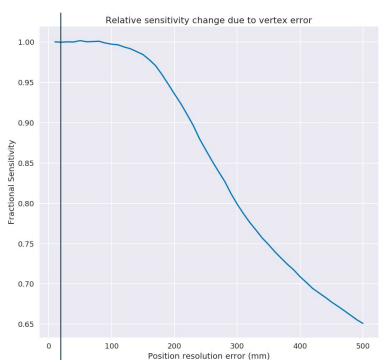
\includegraphics[scale=0.8]{plots/Position} 
	\caption{Relative sensitivity of the ND likelihood analysis as a function of position resolution. Taken from \cite{MorganTalk}.}
	\label{fig:position}
\end{figure}

\subsection{Direction systematics}
A plot describing the fractional sensitivity of our ND analysis liklihood analysis as a function of direction systematics is give in Figure~\ref{fig:direction}. There are a couple of points to make on this plot before continuing. Firstly, it was made under the assumption that no u.R cuts are applied so the angular resolution primarily affects the solar neutrino cut. Secondly, it was made using an analytical model which does not appear to be a good substitute for a numeric pdf. It is assumed this is the reason for the anomalous result in the first bin. Most likely the best way to read this plot is as a fraction from the second bin ($\approx$0.93).

In this case the absolute difference between the fitted scatter tail parameter ($\beta_s$ in \cite{WaterUniDoc}) is quoted on the x-axis. This value is not available in \cite{WaterUniDoc}, where relative differences are quoted in order to form the systematic proposed by \cite{Oser} and used in the SNO LETA paper \cite{LETApaper}. However, the values quoted in Table~7.4 of \cite{WaterUniDoc} can be converted by simply scaling by the mean $\beta_{s,MC}$, or re-running the analysis with the absolute values. Figure~\ref{fig:beta_s_absolute} shows the absolute values for the data - Monte Carlo for each N16 run which passes all the cuts described in \cite{WaterUniDoc}. Taking the weighted mean and standard deviation of those points gives:
\begin{equation}
\beta_{s, absolute} = -0.59 +/- 2.05
\end{equation}
This result can be used to generate the conservative two sided uncertainty as give in Table~\ref{tab:direction}. If we take the conservative assumption that the uncertainty is infact the full range of the two sided uncertainty we get:
\begin{equation}
\Delta_{direction} = 3.2
\end{equation}
Applying $\Delta_{pdirection}$ to Figure~\ref{fig:direction} suggests something on the order of a 2-3\% effect. 

\begin{table}
	\label{tab:direction}
	\centering
	\begin{tabular}{p{2.5cm}|p{3.5cm}}
		\hline
		Systematic &  Value\\
		\hline
		\hline
		$\beta_{s, absolute}$ & -2.6 / +0.6 \\
		\hline
	\end{tabular}
	\caption{Absolute two sided uncertainty on the $\beta_s$ parameter}
\end{table}

\begin{figure}\centering
	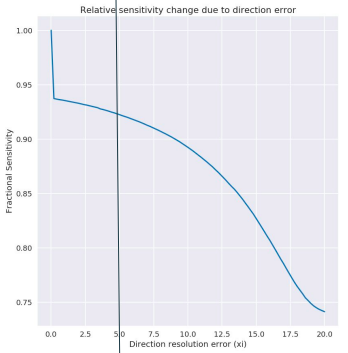
\includegraphics[scale=0.8]{plots/Direction} 
	\caption{Relative sensitivity of the ND likelihood analysis as a function of direction resolution. Taken from \cite{MorganTalk}.}
	\label{fig:direction}
\end{figure}

\begin{figure}\centering
	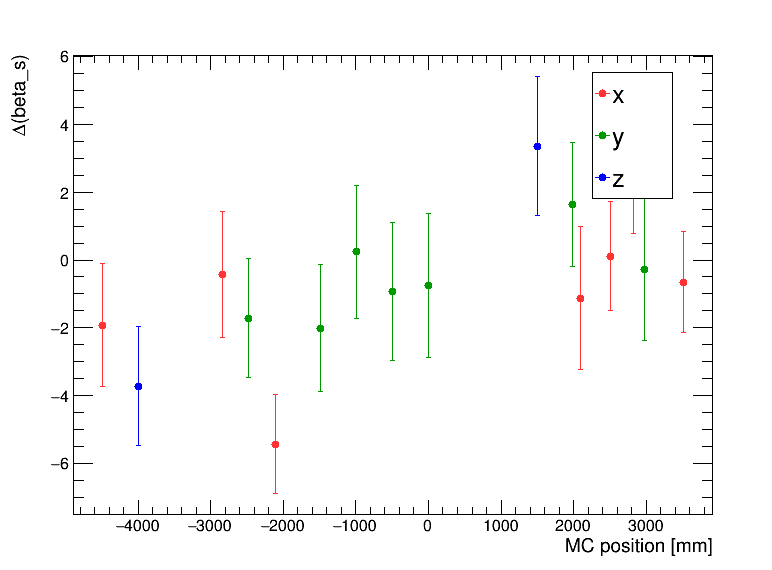
\includegraphics[scale=0.5]{plots/beta_s_absolute} 
	\caption{Absolute differences in the $\beta_s$ parameter for all runs which pass cuts as described in \cite{WaterUniDoc}}
	\label{fig:beta_s_absolute}
\end{figure}

\subsection{Energy systematics}

\begin{figure}\centering
	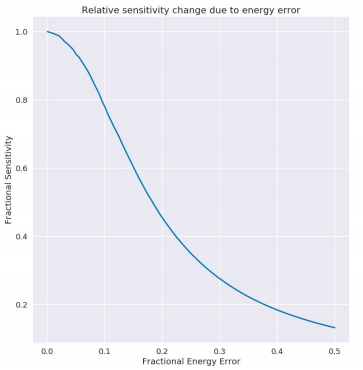
\includegraphics[scale=0.8]{plots/Energy} 
	\caption{Relative sensitivity of the ND likelihood analysis as a function of energy resolution. Taken from \cite{MorganTalk}.}
	\label{fig:energy}
\end{figure}

\section{Conclusions}

\begin{thebibliography}{9}
	\bibitem{MorganTalk} 
	Morgan Askins,
	Reconstruction systematics, 
	\textit{SNO+ document database \#4549}
	
	\bibitem{WaterUniDoc} 
	N. Barros et al,
	\textit{http://nu.hep.upenn.edu/~nfbarros/snoplus/UnidocReleases.html}
	
	\bibitem{Oser}
	S. Oser,
	A comment on Implementing the Angular Resolution Uncertainty in Sigex, 2008
	\textit{SNO internal doc}
	
	\bibitem{LETApaper}
	SNO collaboration,
	Low Energy Threshold Analysis of the Phase I and Phase II Data Sets of the Sudbury Neutrino Observatory
	\textit{arXiv:0910.2984}
\end{thebibliography}

\end{document}
